\documentclass{beamer}
\usetheme{CambridgeUS}


%%% PACKAGES
\usepackage[russian]{babel}
\usepackage[utf8]{inputenc}
\usepackage{amsmath}
\usepackage{amssymb}
\usepackage{tikz}
\usepackage{graphics}
\usepackage{color}
\usepackage{algorithmicx}
\usepackage{algpseudocode}
\usepackage[]{algorithm2e}

%%% BEAMER SETTINGS
\setbeamertemplate{navigation symbols}{}
\setbeamertemplate{headline}{}

%%% TIKZ SETTINGS
\usetikzlibrary{fit}

%%% NEW COMMANDS
\def\pitem{\pause \item}


%\includeonlyframes{current} % leaves only the given frames

\begin{document}
\title[Автоматическая генерация тестов]{Теоретический анализ времени работы эволюционных алгоритмов при генерации тестов}
%\transduration{20}
\author[Денис Антипов]{Денис Антипов}
\institute[Университет ИТМО]{Национальный исследовательский университет информационных технологий, механики и оптики}
\date{13.04.2016}

 
\begin{frame}
 \maketitle
\end{frame}
 
 \begin{frame}{План презентации}
  \tableofcontents
 \end{frame}

 \section{Введение}
 \subsection{Эволюционные алгоритмы}
 \begin{frame}{Эволюционные алгоритмы}
  \begin{itemize}
   \item Алгоритмы оптимизации, использующие идеи эволюции.
   \item При инициализации алгоритма создается первое поколение решений.
   \item На каждой итерации алгоритм генерирует новое поколение на основе предыдущего.
   \item Алгоритм заканчивает работу, когда находит достаточно хорошее решение.
  \end{itemize}
 \end{frame}
 
 \subsection{Генерация тестов}
 \begin{frame}{Мотивация}
  \begin{itemize}
   \item Эволюционные алгоритмы успешно использовались для генерации тестов\footnote{Буздалов М.В. Диссертация на тему «Генерация тестов для определения неэффективных решений олимпиадных задач по программированию с использованием эволюционных алгоритмов»}.
   \item Сложная оценка ожидаемого числа итераций таких алгоритмов.
   \item Для оценки времени работы был выбран алгоритм,генерирующий тесты для конкретной реализации алгоритма Дейкстры.
  \end{itemize}
 \end{frame}
 
 \subsection{Описание алгоритма}
 \begin{frame}{Описание алгоритма}
  \begin{algorithm}[H]
  \KwData{$V$, $E$}
  \KwResult{$graph$ with all the edges relaxed}
  
  $graph \gets init()$
  
  $f \gets dijkstra(graph)$
  
  \While{$f \ne E$}{
    
    $graph' \gets mutate(graph)$
    
    $f' \gets dijkstra(graph')$
    
    \If{$f' \ge f$}{
      $graph, f \gets graph', f'$
    }
  }
 % \Return{$graph$}
  \end{algorithm}
 \end{frame}
 
 \section{Оценка времени работы}
 \subsection{Разреженный граф}
 \begin{frame}{Разреженный граф}
  \begin{itemize}
   \item В случае, когда $V \gg E$, можно считать, что алгоритм не выбирает новый граф, если он нарушает инвариант: все задействованные ребра графа образуют дерево с корнем в стартовой вершине.
   \item Это замедлит алгоритм, но зато позволит дать оценку на время работы:
   \begin{itemize}
    \item Если $V > E + 1$:
    $$T \le \frac{EV(2V - E - 1)}{(E + 1)(V - E - 1}(\gamma + \ln E) - \frac{EV}{V - E - 1} \ln\frac{V - 1}{V - E}$$
    \item Если $V = E + 1$:
    $$T \le \frac{\pi^2 E^2}{6} + o\left( \frac{\pi^2 E^2}{6} \right)$$
   \end{itemize}
   \item Если $V = aE$, где $a > 1$ -- константа, тогда время работы $T \lesssim V \ln{E} \left(2 + 1/(a - 1)\right)$
  \end{itemize}
 \end{frame}

 \subsection{Плотный граф}
 \begin{frame}{Плотный граф}
  Рассмотрим случай графа с двумя вершинами:
  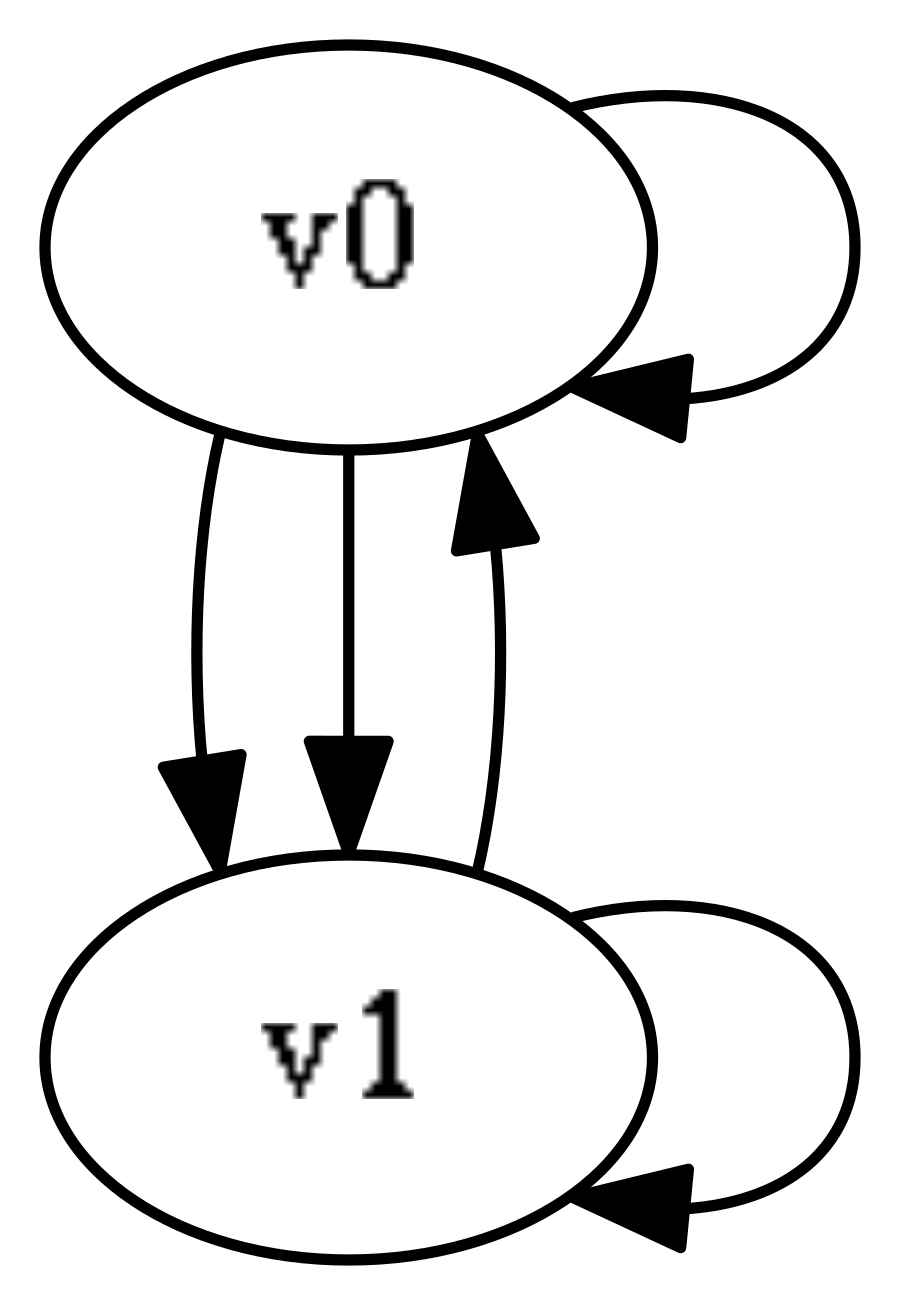
\includegraphics[height=3cm]{pic/2v_graph.png}
  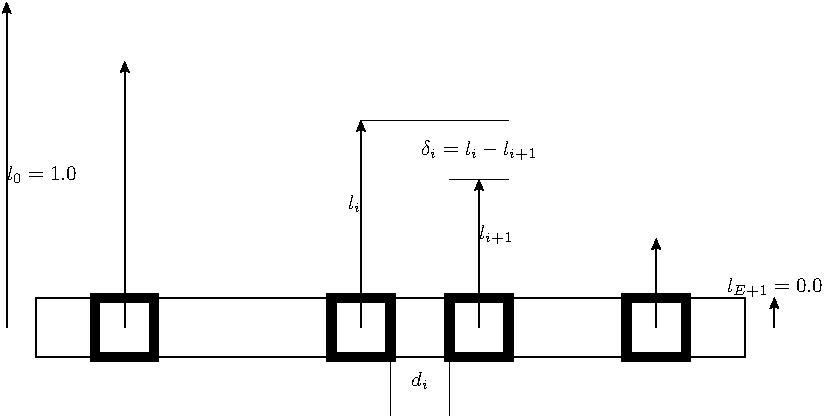
\includegraphics[height=5cm]{pic/edges.pdf}
 \end{frame}
 
  \begin{frame}{Плотный граф}
  \begin{itemize}
   \item Введем потенциал $\Phi = \sum d_i \delta_i$
   \item Матожидание его изменения: $$E(\Phi_t - \Phi_{t + 1}) \ge \sum_{\text{unrelaxed edges}} \frac{1}{E} \frac{1}{4} \delta_i = \frac{1}{4E} \Phi_t$$
   \item По мультипликативной дрифт-теореме: $$E(T) \ge 4E \left( 1 + \ln\frac{\Phi_0}{\Phi_{min}}\right)$$
   \item Проблема: $\Phi_{min}$ может быть сколь угодно мал.
  \end{itemize}
 \end{frame}
 
 \begin{frame}{Плотный граф}
  \begin{itemize}
   \item Если бы $\Phi_{min} = \frac{eE}{e^E}$, то ожидаемое время работы не превышало бы $4E^2$
   \item Рассмотрим вероятность случая, когда $\Phi_{min}$ не становится меньше:
   $$p\left(\Phi_{min} > \frac{eE}{e^E}\right) > p\left(\forall \delta_i > \frac{eE}{e^E}\right) = \prod_{i=1}^E (1 - 2 \frac{eE}{e^E}i) \ge$$
   $$\ge (1 - 2 \frac{eE^2}{e^E})^E \xrightarrow[E \to +\infty]{} 1 $$
  \end{itemize}
 \end{frame}
 
 \section{Эксперименты}
 \subsection{Разреженный граф}
 \begin{frame}{Разреженный граф}
  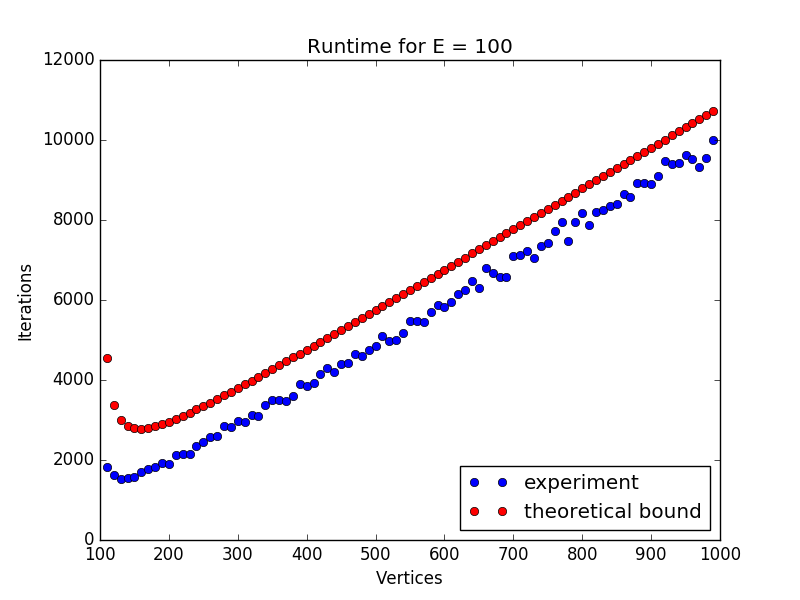
\includegraphics[width=10cm]{pic/rarefied_graph.png}
 \end{frame}
 
 \subsection{Плотный граф}
 \begin{frame}{Плотный граф}
   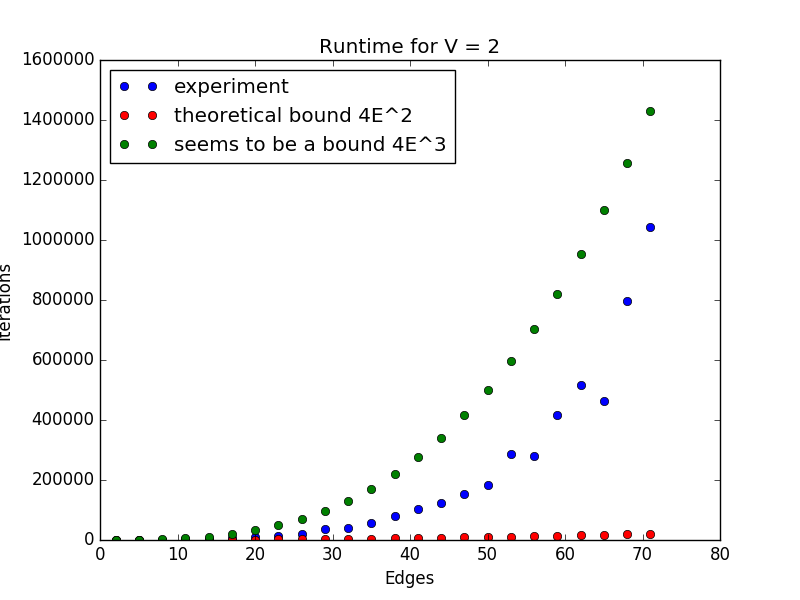
\includegraphics[width=10cm]{pic/dense_graph.png}
 \end{frame}
 
 \section{Заключение}
 \begin{frame}{Дальнейшая работа}
   \begin{itemize}
    \item Исследовать, как влияет на матожидание оставшаяся часть исходов.
    \item Расширить рассуждение на графы с более, чем двумя вершинами.
   \end{itemize}
 \end{frame}
 
 \begin{frame}
  \begin{center}
   \Huge Спасибо!
  \end{center}

 \end{frame}


\end{document}